\label{chapter:metodo}

Este capítulo tem o objetivo de descrever a solução proposta neste trabalho, visando localizar e identificar objetos
em ambientes confinados utilizando leitores e etiquetas passivas RFID, para gerenciamento e controle de bens.
%
Esta solução pode ser aplicada, por exemplo, para o controle e levantamento de patriminio de universidades.

%
%
\section{Visão geral do método}

O método consiste em um sistema que localiza qualquer objeto que tenha uma etiqueta RFID passiva fixada em seu corpo,
as etiquetas serão localizadas e identificadas a medida em que transitam de uma sala para outra em um edifício.
%
A localização e identificação é feita por meio de leitores RFID, módulo wireless, e micro-controlador colocados próximos às portas da sala
de um prédio, assim os leitores devem ler as tags que passam pela porta, bem como, o módulo wireless irá propagar está informação via
comunicação com um servidor web.


Cada leitor RFID junto ao controlador será responsável por uma sala, portanto qualquer etiqueta lida por aquele leitor
ocasionará nas ações referentes a mesma sala. As ações poderá ser de atualização sobre a localização do objeto ou informando
que o objeto está em transição para outra sala no edifício.
\begin{figure}[H]
              \caption{\label{fig:modelo}{Modelo Proposto}}
              \centering
              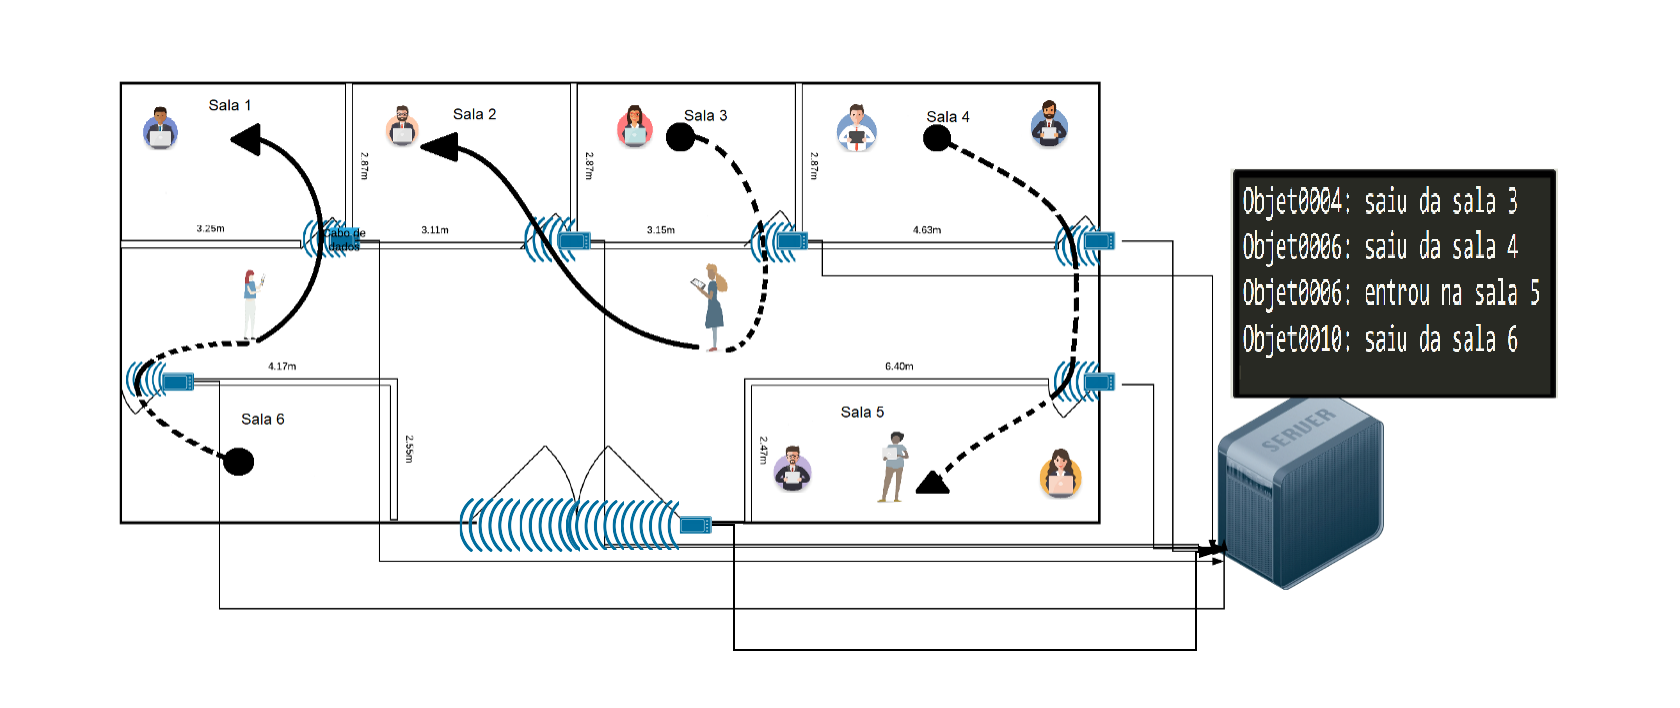
\includegraphics[width=1.1\textwidth]{Figuras/bigpicture.png}
              \legend{Fonte: Própria}
        \end{figure}

\par
Na \autoref{fig:modelo} é possível notar que há um dispositivo acoplado próximo a
porta de cada sala, esse dispositivo contém o leitor RFID, esse dispositivo será encarregado de consultar um
servidor para assim tomar decisões do que será feito com o status do objeto, cada objeto possui uma tag RFID fixada
nele e quando passar pela porta o leitor identifica o objeto e altera sua as informações sobre sua localização.

\par
O método proposto consiste basicamente nas seguintes etapas:
\begin{enumerate}
    \item Identificação dos objetos que serão rastreados;
    \item Monitoramento e localização dos objetos rastreáveis em ambiente indoor; e
    \item Configuração de controle e monitoramento de transição dos objetos.
\end{enumerate}

%
%
\section{Identificação dos objetos rastreáveis}

Antes de qualquer passo, e visando a implantação do sistema proposto, é necessário a identificação dos objetos.
Nessa etapa é anexado ao objetos as etiquetas RFID e realizada uma descrição do objeto portador dessa etiqueta
no sistema, para que ao entrar e sair das salas do edifício além de fornecer a localização do objeto também seja
possível ter detalhes sobre aquele objeto, dessa forma se objeto tiver uma registro local isso irá constar na
descrição do objeto. Essa etapa pode ser considerada como a fase de cadastro do objeto.

\begin{figure}[H]
              \caption{\label{fig:objeto}{Objeto com tag RFID}}
              \centering
              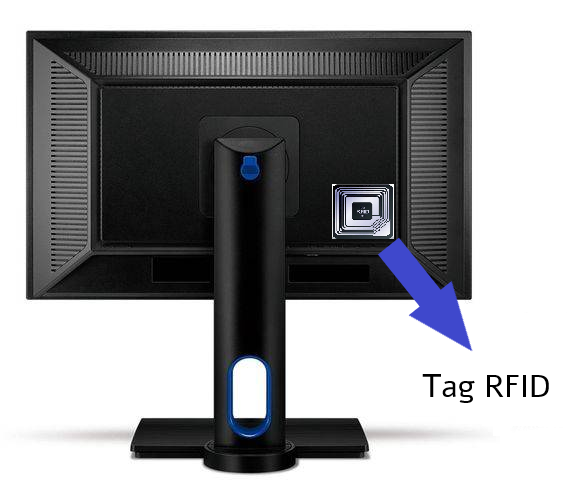
\includegraphics[width=0.4\textwidth]{Figuras/monitor.png}
              \legend{Fonte: Própria}
\end{figure}
\par
Na \autoref{fig:objeto} é apresentado um objeto com uma tag RFID passiva anexada em seu corpo, todos os objetos que serão rastreáveis no sistemas possuirão uma tag RFID anexada da mesma forma.

%
\section{Monitoramento e Localização dos objetos rastreáveis}

O monitoramento é realizado pelo sensor de RFID que estará em cada porta das salas do prédio e será responsável
identificar o objeto e repassar esta informação ao módulo wireless que irá enviar para um servidor web sobre as
ocorrências/transições das salas. Assim, criando um log sobre transição de cada objeto, provendo ao usuário do sistema
alertas para que decisões necessárias sejam tomadas.

%\todo[inline,color=red]{Sugiro descrever aquela ideia de dizer que além das transições entre as salas também é possível identificar
%aproximadamente a posição na sala. Como seria isto?}


\subsection{Fluxo de execução do método em cada sala}
Os dispositivos de cada sala terão o seguinte fluxo de execução apresentado na \autoref{fig:fluxograma},
o fluxo exemplifica as tarefas que cada dispositivo executará. Neste fluxograma, os retângulos representam
processos e os retângulos com bordas duplas processos pré-definidos, os losangos representam as tomadas de decisões,
os ícones com bordas curvas para o mesmo lado representam operações nos dados do sistema e o ícone com bordas curvas
opostas representam o início do fluxo.

\begin{figure}[H]
              \caption{\label{fig:fluxograma}{Fluxograma de cada sala}}
              \centering
              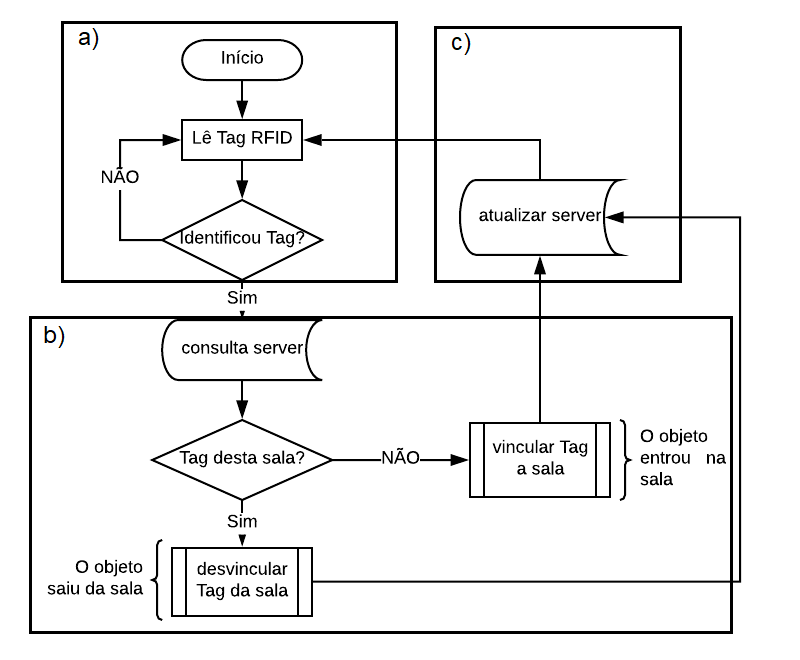
\includegraphics[width=1\textwidth]{Figuras/fluxograma.png}
              \legend{Fonte: Própria}
\end{figure}

\par
O fluxograma é separado em três módulos: \textbf{a}, \textbf{b} e \textbf{c}. O módulo \textbf{a} é onde é realizado o
monitoramento da da sala, realizando leituras dos objetos que entram e saem da sala, no módulo \textbf{b} é o onde serão
tomadas as decisões referente a etiqueta anexada ao objeto lida naquele momento, verificando se a etiqueta está ou não
localizada naquela sala e processando as alterações necessárias. O módulo \textbf{c} é o último processo que atualiza as
informações do servidor para que os dados consultados sejam iguais para todos.


\subsection{Localização dos objetos}

Os objetos serão localizado no sistema baseado nos algoritmos de proximidade, ou seja, a partir do momento em que o leitor
RFID identifica uma etiqueta, esse objeto terá a localização referente àquele leitor, nesse sistema os leitores irão representar
salas, portanto a localização indicará que o objeto estará na sala cujo o leitor que realizou a leitura representa.

%\par\todo[color=green]{Sugiro descrever mais sobre este servidor web, exemplo de conexão local ou não, banco de dados e
%outras informações necessárias}
O sistema conterá um servidor web desenvolvido utilizando Node.js, que estará conectado à mesma rede LAN (local area network) que os dispositivos de porta, o mesmo possuirá uma base de dados sendo o sistema de gerenciamento de dados o MongoDB, para armazenar informações e detalhes de cada objeto e tal servidor será responsável por tratar problemas relacionados a leituras de uma mesma etiqueta mais de uma vez,
o papel do servidor é de grande importância também sendo utilizado para consultar informações referentes aos objetos.


\section{Configuração de controle e monitoramento de transição dos objetos}

Para um melhor gerenciamento dos objetos, o sistema conta com alertas para que caso um objeto inicie uma transição
para outra sala e nesse trajeto o objeto não entre em nenhuma sala excedendo um tempo determinado, um alerta é gerado
informado que o objeto não entrou em nenhuma sala do edifício até o momento da geração do alerta.

\par
Um tempo padrão deve ser configurado para os alertas, se um objeto exceder esse tempo na transição um alerta é gerado no servidor.
O tempo deve ser configurado na implantação do sistema. Um outro alerta que pode ser criado seria no caso de
ser definido uma área de limite para alguns objetos e ele sejam deslocados para fora dessa área delimitada.

\par
Cada transição de objeto também será armazenada nos logs do sistema com data e hora, sala que saiu ou entrou, para que
os eventos ocorridos sejam registrados e possua mais um recurso na consulta para caso ocorra falhas.
%\todo[inline,color=green]{Sugiro descrever um pouco mais, talvez falar que com os dados de log das
%transições do sistema é possível também delimitar
%salas que objetos não podem sair, ou não podem entrar, criando zonas de controle.}


\section{Conexão dos dispositivos de porta com o servidor e energia}
A comunicação entre os dispositivos da porta com o servidor acontecerá por meio de uma WLAN, ou seja todos estarão em uma rede
local e assim poderão se comunicar, entretanto a comunicação será diretamente entre um dispositivo e o servidor,
não havendo comunicação entre dois dispositivos. O Arduino nano contará com um módulo ESP-8266, esse módulo possibilita a
conexão com uma rede wireless 802.11 b/g/n.
%\todo[color=green]{Falar um pouco sobre baixo consumo de energia}.

\par
O Arduino nano opera em uma voltagem de 5V de energia contínua, um consumo relativamente baixo em relação as outros dispositivos eletrônicos e as tag passivas não possuem alimentação, elas são alimentadas apenas pela energia eletromagnética emitida pelos leitores RFID, esses dois quesitos tornam o protótipo ainda mais viável, pois isso é um fator positivo visto que o custo pós implantação não é alto.


\section{Modelo de Prototipação}

O protótipo a ser desenvolvido neste trabalho é composto pelo servidor web que nesse primeiro instante será um computador de
propósito geral e pelo dispositivo da porta, que será um Arduino Nano ATmega168 junto ao leitor RFID RC522 e módulo ESP8266 (módulo wireless).
O leitor RFID pode ser visto na \autoref{fig:leitorRFID}, esse leitor é capaz de ler etiquetas que operam em
frequências de 13,56 Mhz.
\begin{figure}[H]
              \caption{\label{fig:leitorRFID}{Leitor RFID RC522}}
              \centering
              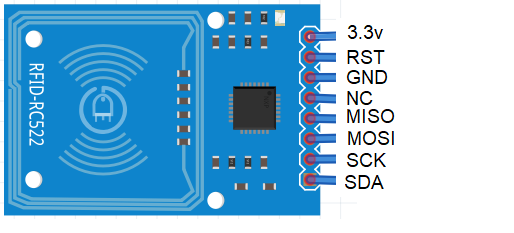
\includegraphics[width=0.7\textwidth]{Figuras/rfid_rc522.PNG}
              \legend{Fonte: Fritzing}
\end{figure}

\par
O leitor RFID utiliza a interface SPI (\textit{Serial Peripheral Interface} ) para comunicação com o Arduino,
essa conexão é síncrona e é realizada por meio dos pinos de $9$ à $13$. A prototipagem entre o Arduino e o leitor RFID
segue o esquema abaixo que também pode ser visto na \autoref{fig:esq_conexoes}:
\begin{itemize}
    \item 3.3V - conectado ao pino de 3.3v no Arduino, essa conexão faz a alimentação do leitor RFID;
    \item RST (\textit{Reset})- conectado ao pino 9 do Arduino;
    \item GND (\textit{graduated neutral density filter}) - conectado ao pino GND do Arduino;
    \item NC/IRQ (\textit{Interrupt Request})- não utilizado;
    \item MISO (\textit{Master In Slave Out}) - conectado ao pino 12;
    \item MOSI  (\textit{Master Out Slave In}) - conectado ao pino 11;
    \item SCK  (\textit{Serial Clock}) - conectado ao pino 13;
    \item SDA/ SS (\textit{Serial Data Line/ Select Slave}) - conectado ao pino 10.
\end{itemize}

%\todo[inline,color=green]{Sugiro descrever a função de cada um dos pinos acima.}

\begin{figure}[H]
              \caption{\label{fig:moduloWii}{Módulo Wifi ESP8266}}
              \centering
              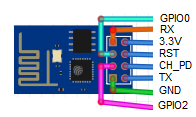
\includegraphics[width=0.6\textwidth]{Figuras/Modulo_ESP8266.png}
              \legend{Fonte: Fritzing}
\end{figure}

\par
O ESP8266 é um módulo que permite a conexão do Arduino com redes wireless 802.11 b/g/n, esse módulo pode
trabalhar em dois modos tanto como ponto de acesso ou no modo estação que envia e recebe dados.
%\todo[color=green]{Descrever}.
\begin{itemize}
    \item GND (\textit{graduated neutral density filter}) - conectado ao pino GND do Arduino;
    \item GPIO0 (\textit{General Purpose Input/Output}) - não conectado ;
    \item GPIO2 (\textit{General Purpose Input/Output})- não conectado ;
    \item TX (\textit{Transmission}) - conectado ao pino digital 2 no Arduino;
    \item RX (\textit{Received})- conectado ao pino digital 3 no Arduino junto com dois resistores um de 220$\Omega$ e outro de 330$\Omega$ para dividir a tensão;
    \item RST (\textit{Reset}) - não conectado ;
    \item CH\_PD (\textit{Chip enable}) - conectado ao pino 3.3v mas com resistor de 10 $K\Omega$.
\end{itemize}

%\todo[inline,color=green]{Descrever a função dos pinos}

\begin{figure}[H]
              \caption{\label{fig:esq_conexoes}{Esquema de Conexões}}
              \centering
              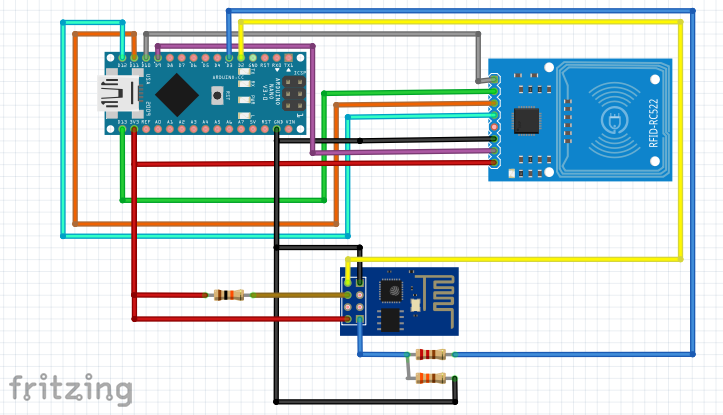
\includegraphics[width=1\textwidth]{Figuras/esquema_de_conexoes2.PNG}
              \legend{Fonte: Própria}
\end{figure}


